
\section{End-to-End Evaluation}
\label{sec:e2e}

In Figure~\ref{fig:e2e} we compare the end-to-end performance of \Sys to key baselines, including our own implementation of ordinary speculative decoding, as well as the strongest open source inference engines (vLLM/SGLang).\footnote{We find SGLang usually outperforms vLLM, so we use it as the main baseline throughout.}
We also include EAGLE-3 when supported by open source engines.\footnote{In our experiments Llama-3.2-1B outperforms Eagle-3 as a draft model for Llama-3.1-70B in SGLang.}
We attain almost a 5x speedup on average compared to our autoregressive baseline, and are up to twice as fast as the optimized speculative decoding baselines, establishing a new state of the art. 

Though speculative decoding algorithms are designed to trade off compute for lower latency, we show in Figure~\ref{fig:e2e} (right) that SSD pushes the Pareto frontier across both latency and throughput, with the biggest gains at lower batch sizes.
This means that SSD does not just improve the best possible decoding speed, \textit{but is also more compute efficient per device.}

% Though SSD is designed to trade off compute for lower latency, it nonetheless pushes the Pareto frontier across both latency and throughput, with biggest gains at lower batch sizes where the draft model is not yet compute-bound. This means that SSD does not just improve the best possible decoding speed, but is also more compute efficient per device. 

\begin{figure}[ht]
    \centering
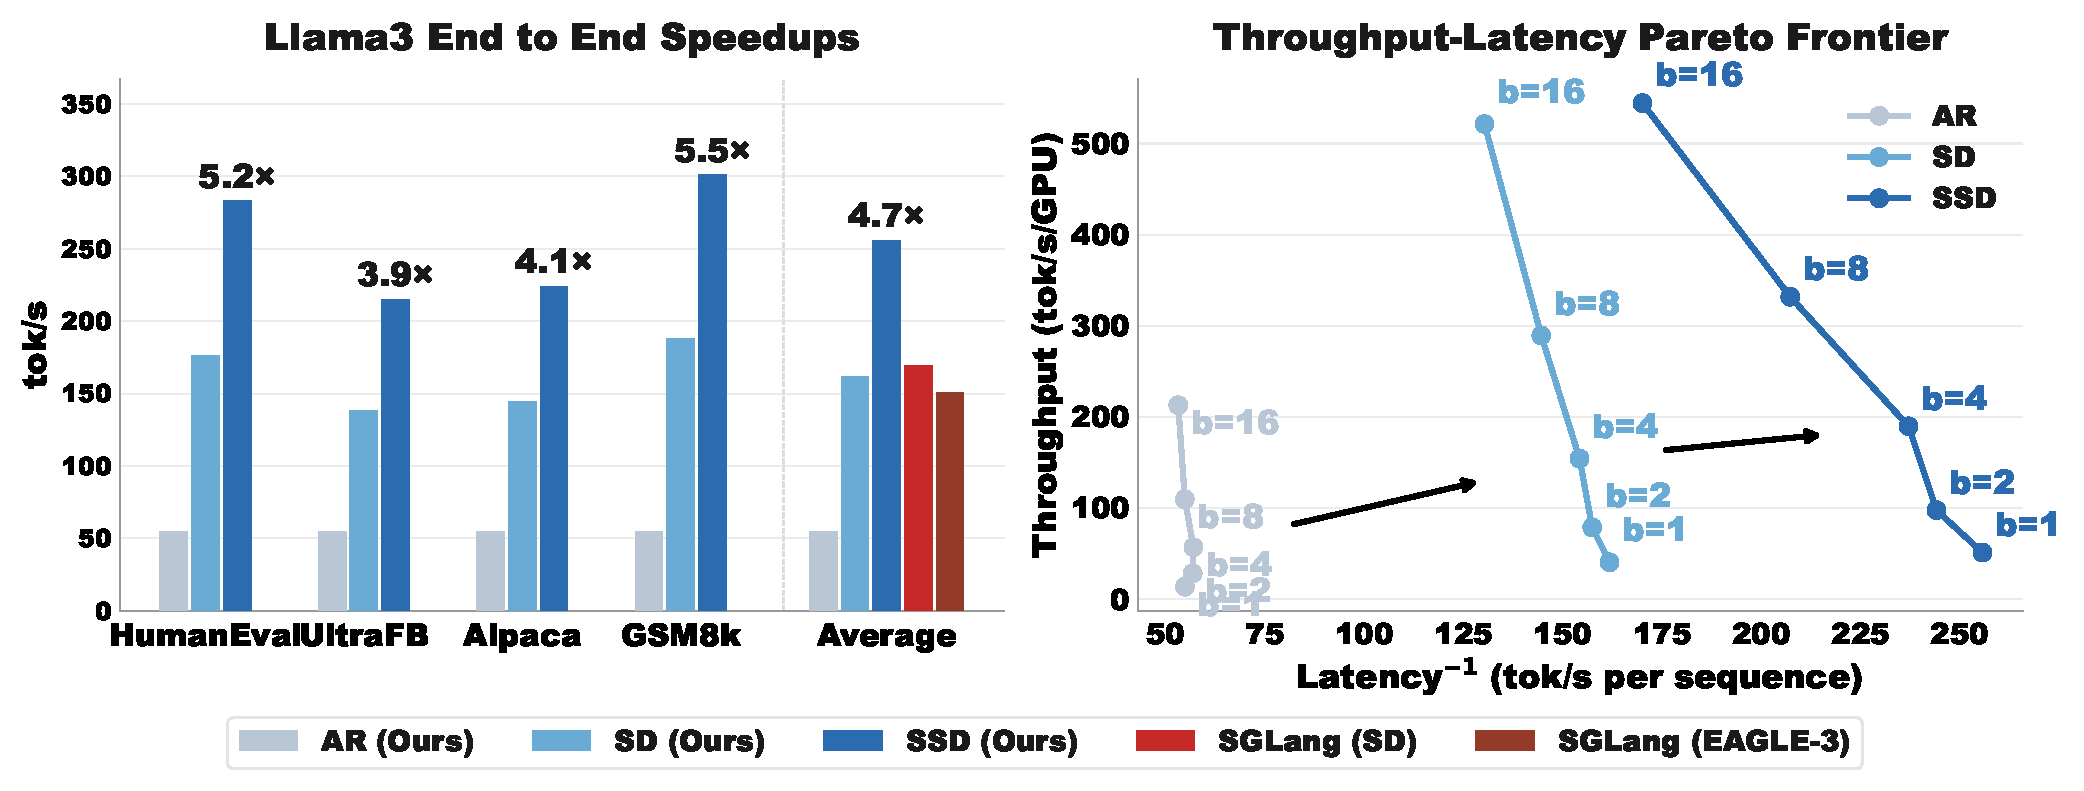
\includegraphics[width=\linewidth]{figures/llama_e2e_pareto.pdf}
    \caption[End-to-end decoding speed comparison.]{
    (Left) End-to-end decoding speed comparison of SSD compared to SD and standard autoregressive decoding on Llama-3.1-Instruct 70B across four datasets. (Right) SSD improves the throughput-latency Pareto frontier.\protect
    }
    \label{fig:e2e}
\end{figure}


\section{Conclusion and Limitations}

Speculative decoding trades compute for latency, but drafting and verification remain synchronous. We introduce speculative speculative decoding (SSD), which parallelizes even this sequential dependence. We derive performance bounds, study each component of the design space, and distill our findings into \Sys, an optimized SSD algorithm which achieves up to 2x speedup over optimized speculative decoding and up to 5x over autoregressive generation across datasets and model families.


Speculative decoding focuses on reducing latency, and is generally ineffective for throughput-bound workloads---large-scale RL, offline data generation---since it adds verification workload to an already compute-bound process.
Nonetheless, we show that SSD is able to push the latency-throughput Pareto frontier, leading to gains in both latency \textit{and} throughput, even after taking into account the additional hardware used.
% Speculative decoding aims toward low latency potentially at the cost of performance on throughput-bound workloads---large-scale RL, offline data generation---since the draft model may do unnecessary work pre-emptively.
% Despite this, SSD outperforms SD even when adjusted for the additional hardware used, and pushes the Pareto frontier of latency-throughput. 

Much remains open.
SSD composes naturally with EAGLE and token-tree speculation (Appendix~\ref{app:combine}); the joint design and tradeoff space is largely unexplored.
Latency can be further reduced by scaling the number of draft devices and thus the speculation cache, though the returns will eventually diminish.
Finally, sharing speculation endpoints across several target model deployments at the cluster level---similar to prefill-decode disaggregation~\citep{disagg}---is another natural direction.
% Finally, because draft models in the SSD framework become compute-bound faster than those under SD, disaggregation of drafting and verification at cluster scale~\citep{disagg} is a natural next step. 

\color{black}
